% Options for packages loaded elsewhere
\PassOptionsToPackage{unicode}{hyperref}
\PassOptionsToPackage{hyphens}{url}
%
\documentclass[
  14pt,
  ignorenonframetext,
  aspectratio=169,
]{beamer}
\usepackage{pgfpages}
\setbeamertemplate{caption}[numbered]
\setbeamertemplate{caption label separator}{: }
\setbeamercolor{caption name}{fg=normal text.fg}
\beamertemplatenavigationsymbolsempty
% Prevent slide breaks in the middle of a paragraph
\widowpenalties 1 10000
\raggedbottom

\usepackage{amsmath,amssymb}
\usepackage{iftex}
\ifPDFTeX
  \usepackage[T1]{fontenc}
  \usepackage[utf8]{inputenc}
  \usepackage{textcomp} % provide euro and other symbols
\else % if luatex or xetex
  \usepackage{unicode-math}
  \defaultfontfeatures{Scale=MatchLowercase}
  \defaultfontfeatures[\rmfamily]{Ligatures=TeX,Scale=1}
\fi
\usepackage{lmodern}
\usetheme[]{monash}
\ifPDFTeX\else  
    % xetex/luatex font selection
\fi
% Use upquote if available, for straight quotes in verbatim environments
\IfFileExists{upquote.sty}{\usepackage{upquote}}{}
\IfFileExists{microtype.sty}{% use microtype if available
  \usepackage[]{microtype}
  \UseMicrotypeSet[protrusion]{basicmath} % disable protrusion for tt fonts
}{}
\makeatletter
\@ifundefined{KOMAClassName}{% if non-KOMA class
  \IfFileExists{parskip.sty}{%
    \usepackage{parskip}
  }{% else
    \setlength{\parindent}{0pt}
    \setlength{\parskip}{6pt plus 2pt minus 1pt}}
}{% if KOMA class
  \KOMAoptions{parskip=half}}
\makeatother
\usepackage{xcolor}
\newif\ifbibliography
\setlength{\emergencystretch}{3em} % prevent overfull lines
\setcounter{secnumdepth}{-\maxdimen} % remove section numbering


\providecommand{\tightlist}{%
  \setlength{\itemsep}{0pt}\setlength{\parskip}{0pt}}\usepackage{longtable,booktabs,array}
\usepackage{calc} % for calculating minipage widths
\usepackage{caption}
% Make caption package work with longtable
\makeatletter
\def\fnum@table{\tablename~\thetable}
\makeatother
\usepackage{graphicx}
\makeatletter
\def\maxwidth{\ifdim\Gin@nat@width>\linewidth\linewidth\else\Gin@nat@width\fi}
\def\maxheight{\ifdim\Gin@nat@height>\textheight\textheight\else\Gin@nat@height\fi}
\makeatother
% Scale images if necessary, so that they will not overflow the page
% margins by default, and it is still possible to overwrite the defaults
% using explicit options in \includegraphics[width, height, ...]{}
\setkeys{Gin}{width=\maxwidth,height=\maxheight,keepaspectratio}
% Set default figure placement to htbp
\makeatletter
\def\fps@figure{htbp}
\makeatother

% Packages
\usepackage{amsmath, bm, amssymb, amsthm, mathrsfs,pifont,accents,mathtools,relsize,makecell}
%\usepackage{enumitem,calc}
\usepackage[bb=boondox]{mathalfa}
\usepackage{url}
\usepackage{multirow, booktabs, float, textcmds, siunitx}
\usepackage{bm,booktabs,animate,ragged2e,multicol,microtype,hyperref}
\usepackage{array,ifthen,colortbl,adjustbox}

% Colors
\definecolor{shadecolor}{RGB}{225,225,225}
\definecolor{DarkBrown}{RGB}{80,70,60}
\setbeamercolor{description item}{fg=Orange}
\setbeamercolor{block title alerted}{fg=white,bg=DarkBrown}
\setbeamercolor{block title}{fg=white,bg=DarkBrown}
\setbeamercolor{frametitle}{bg=DarkBrown,fg=white}

\definecolor{newred}{rgb}{0.8,0,0}
\definecolor{avocado}{HTML}{2B7A0B}
\definecolor{newblue}{HTML}{0270c0}
%\definecolor{DarkGray}{RGB}{33,33,33}
%\definecolor{LightGray}{RGB}{150,150,150}
%\definecolor{LightGray2}{RGB}{200,200,200}
%\definecolor{Ocean}{RGB}{129,194,234}
%\definecolor{DarkOrange}{RGB}{255, 152, 0}
\definecolor{LightOrange}{RGB}{255, 193, 7}
%\definecolor{DarkGreen}{RGB}{91, 141, 8}
%\definecolor{LightGreen}{RGB}{122, 188, 12}
%\definecolor{LightPurple}{RGB}{191, 83, 219}
%\definecolor{DarkPurple}{RGB}{142, 36, 170}
%\definecolor{VeryLightGray}{RGB}{249, 249, 249}
%\definecolor{mybluehl}{HTML}{cbd3ff}

\newcolumntype{M}[1]{>{\centering\arraybackslash}m{#1}}
\newcolumntype{L}[1]{>{\raggedright\arraybackslash}m{#1}}
\newcolumntype{R}[1]{>{\raggedleft\arraybackslash}m{#1}}
\newcolumntype{P}[1]{>{\centering\arraybackslash}p{#1}}
\renewcommand<>\rowcolor[1]{\only#2{\\[-\normalbaselineskip]\beameroriginal\rowcolor{#1}}}
\renewcommand<>\cellcolor[1]{\only#2{\beameroriginal\cellcolor{#1}}}

% Figures
\graphicspath{{figs/}}

% Fonts
\usepackage{fontawesome}

% Monash title page
\setbeamertemplate{title page}
{\placefig{-0.01}{-0.01}{width=1.01\paperwidth,height=1.01\paperheight}{figs/stones.png}
\placefig{0.2}{8}{width=4cm}{monash_bw}
\begin{textblock}{10.5}(.5,0.3)
\fontsize{24}{26}\selectfont\bfseries\sffamily\textcolor[RGB]{204,89,0}{\inserttitle}\\[0.3cm]
\fontsize{12}{12}\selectfont\bfseries\sffamily\textcolor[RGB]{204,89,0}{\insertsubtitle}
\end{textblock}
\begin{textblock}{7.5}(.5,6.9)
\fontsize{13}{13}\selectfont\sffamily\textcolor[RGB]{232,201,175}{\bfseries\insertauthor}
\end{textblock}
\begin{textblock}{4.2}(11.6,8.3)\pgfsetfillopacity{0.75}
\begin{beamercolorbox}[wd=4.3cm,ht=0.35cm,dp=0.2cm]{block body}
\fontsize{10}{10}\sf\color[RGB]{80,70,60}~~\texttt{\href{https://robjhyndman.com/ctprob}{robjhyndman.com/ctprob}}
\end{beamercolorbox}
\end{textblock}
\begin{textblock}{6.2}(0,8.8)\pgfsetfillopacity{0.65}
\begin{beamercolorbox}[wd=4.7cm]{block body}
\fontsize{6}{6}\sf\color[RGB]{72,45,34}~Photo by \href{https://unsplash.com/@edvardr?utm_source=unsplash&amp;utm_medium=referral&amp;utm_content=creditCopyText}{Edvard Alexander Rølvaag} on \href{https://unsplash.com/s/photos/hierarchy?utm_source=unsplash&amp;utm_medium=referral&amp;utm_content=creditCopyText}{Unsplash}
\end{beamercolorbox}
\end{textblock}}

% No section contents
\AtBeginSection[]{}

%\renewenvironment{Shaded}{\color{black}\begin{snugshade}\color{black}}{\end{snugshade}\columnbreak}

% Tikz plots

\usepackage{tikz}
\usepackage{forest}

\usetikzlibrary{trees,shapes,arrows,matrix,shadows,positioning}
\usetikzlibrary{decorations.pathreplacing, arrows, calc, fit, arrows.meta, decorations.pathmorphing, decorations.markings}

\tikzstyle{decision} = [diamond, draw, fill=blue!20,
    text width=4.5em, text badly centered, node distance=4cm, inner sep=0pt]
\tikzstyle{block} = [rectangle, draw, fill=blue!20,
    text width=5cm, text centered, rounded corners, minimum height=4em]
\tikzstyle{line} = [draw, thick, -latex']
\tikzstyle{cloud} = [draw, ellipse,fill=red!20, node distance=3cm,
    minimum height=2em, text centered]
\tikzstyle{connector} = [->,thick]

\tikzset{
  basic/.style = {draw, text width=2cm, drop shadow, font=\sffamily, rectangle},
  root/.style = {basic, text width=3cm, rounded corners=2pt, thin, align=center, fill=red!30},
  level 2/.style = {basic, rounded corners=6pt, thin,align=center, fill=green!60, text width=4em},
  level 3/.style = {basic, thin, align=left, fill=pink!60, text width=1.5em}
  level 2a/.style = {basic, rounded corners=2pt, thin,align=center, fill=blue!50, text width=7em},
  level 2b/.style = {basic, rounded corners=2pt, thin,align=center, fill=green!50, text width=7em},
  level 3a/.style = {basic, rounded corners=2pt, thin, align=center, fill=blue!30, text width=4em},
  level 3b/.style = {basic, rounded corners=2pt, thin, align=center, fill=green!30, text width=4em},
  level 4a/.style = {basic, rounded corners=2pt, thin, align=left, fill=blue!10, text width=3.5em},
  level 4b/.style = {basic, rounded corners=2pt, thin, align=left, fill=green!10, text width=3.5em},
}
\newcommand{\relation}[3]
{
	\draw (#3.south) -- +(0,-#1) -| ($ (#2.north) $)
}
\newcommand{\relationW}[2]
{
	\draw (#2.west) -| ($ (#1.north) $)
}
\newcommand{\relationE}[2]
{
	\draw (#2.east) -| ($ (#1.north) $)
}

\newcommand{\relationD}[3]
{
	\draw (#3.east) -- +(#1,0) |- (#2.west)
}

\pgfdeclareimage[height=0.65cm]{ngreen}{figs/boot/ngreen.pdf}
\pgfdeclareimage[height=0.65cm]{nblue}{figs/boot/nblue.pdf}
\pgfdeclareimage[height=0.65cm]{nred}{figs/boot/nred.pdf}
\pgfdeclareimage[height=0.65cm]{nblack}{figs/boot/nblack.pdf}

% My definitions

\def\E{\text{E}}
\def\V{\text{Var}}
\def\bY{\bm{y}}
\def\by{\bm{y}}
\def\bS{\bm{S}}
\def\bG{\bm{G}}
\def\bI{\bm{I}}
\def\bJ{\bm{J}}
\def\bSigma{\bm{\Sigma}}
\def\bLambda{\bm{\Lambda}}
\def\Var{\text{Var}}
\def\var{\text{Var}}
\newcommand{\btwocol}{\begin{multicols}{2}}
\newcommand{\etwocol}{\end{multicols}}
\def\checkmark{\tikz\fill[scale=0.4](0,.35) -- (.25,0) -- (1,.7) -- (.25,.15) -- cycle;}
\makeatletter
\@ifpackageloaded{caption}{}{\usepackage{caption}}
\AtBeginDocument{%
\ifdefined\contentsname
  \renewcommand*\contentsname{Table of contents}
\else
  \newcommand\contentsname{Table of contents}
\fi
\ifdefined\listfigurename
  \renewcommand*\listfigurename{List of Figures}
\else
  \newcommand\listfigurename{List of Figures}
\fi
\ifdefined\listtablename
  \renewcommand*\listtablename{List of Tables}
\else
  \newcommand\listtablename{List of Tables}
\fi
\ifdefined\figurename
  \renewcommand*\figurename{Figure}
\else
  \newcommand\figurename{Figure}
\fi
\ifdefined\tablename
  \renewcommand*\tablename{Table}
\else
  \newcommand\tablename{Table}
\fi
}
\@ifpackageloaded{float}{}{\usepackage{float}}
\floatstyle{ruled}
\@ifundefined{c@chapter}{\newfloat{codelisting}{h}{lop}}{\newfloat{codelisting}{h}{lop}[chapter]}
\floatname{codelisting}{Listing}
\newcommand*\listoflistings{\listof{codelisting}{List of Listings}}
\makeatother
\makeatletter
\makeatother
\makeatletter
\@ifpackageloaded{caption}{}{\usepackage{caption}}
\@ifpackageloaded{subcaption}{}{\usepackage{subcaption}}
\makeatother
\ifLuaTeX
  \usepackage{selnolig}  % disable illegal ligatures
\fi
\usepackage[]{biblatex}
\addbibresource{hts.bib}
\IfFileExists{bookmark.sty}{\usepackage{bookmark}}{\usepackage{hyperref}}
\IfFileExists{xurl.sty}{\usepackage{xurl}}{} % add URL line breaks if available
\urlstyle{same} % disable monospaced font for URLs
\hypersetup{
  pdftitle={Probabilistic cross-temporal forecast~reconciliation},
  pdfauthor={Rob J Hyndman},
  hidelinks,
  pdfcreator={LaTeX via pandoc}}

\title{Probabilistic cross-temporal forecast~reconciliation}
\author{Rob J Hyndman}
\date{}

\begin{document}
\frame{\titlepage}
\begin{frame}{Forthcoming paper}
\phantomsection\label{forthcoming-paper}
\placefig{0}{1.1}{height=8.3cm, width=20cm}{IJFcover}

\begin{textblock}{8}(7, 1.2)\fontsize{13}{14}\sf
\begin{itemize}\tightlist
\item Girolimetto, Athanasopoulos, Di~Fonzo, Hyndman (2024)
``Cross-temporal probabilistic forecast reconciliation: Methodological and practical issues''.
\item Preprint at \texttt{\href{https://robjhyndman.com/ctprob}{robjhyndman.com/ctprob}}
\end{itemize}
\end{textblock}

\placefig{7}{6.2}{trim = 0 40 0 0, clip=TRUE, width=10cm, height=2.9cm}{danielegiro}
\placefig{10}{6.2}{trim = 0 40 0 0, clip=TRUE, width=10cm, height=2.9cm}{george}
\placefig{13}{6.2}{trim = 0 0 0 30, clip=TRUE, width=10cm, height=2.9cm}{tommy}
\end{frame}

\section{Australian tourism
forecasting}\label{australian-tourism-forecasting}

\begin{frame}{Australian tourism regions}
\phantomsection\label{australian-tourism-regions}
\placefig{0.1}{1.2}{height=7.8cm, width=16cm}{aus_map}
\begin{textblock}{6.5}(9.1,1.4)
\begin{block}{}%\fontsize{12}{13}\sf
  \begin{itemize}\itemsep=0cm\parskip=0cm
    \item Monthly data on visitor night from 1998 -- 2017
    \item From \textit{National Visitor Survey}, annual interviews of 120,000 Australians aged 15+.
    \item Geographical hierarchy split by
    \begin{itemize}
    \item 7 states
    \item 27 zones
    \item 75 regions
    \end{itemize}
  \end{itemize}
\end{block}
\end{textblock}
\end{frame}

\begin{frame}{Australian tourism data}
\phantomsection\label{australian-tourism-data}
\only<1>{\placefig{0.1}{1.4}{width=15.8cm}{tourism1}}
\only<2>{\placefig{0.1}{1.4}{width=15.8cm}{tourism2}}
\only<3>{\placefig{0.1}{1.4}{width=15.8cm}{tourism3}}
\only<4>{\placefig{0.1}{1.4}{width=15.8cm}{tourism4}}
\only<5>{\placefig{0.1}{1.3}{width=15.8cm}{tourism5}}
\end{frame}

\section{Cross-temporal aggregation
constraints}\label{cross-temporal-aggregation-constraints}

\begin{frame}{Coherent cross-temporal forecasts}
\phantomsection\label{coherent-cross-temporal-forecasts}
\alert{What we want}

\begin{itemize}
\tightlist
\item
  We want forecasts of all series at all levels of cross-sectional
  aggregation.
\item
  We want forecasts at monthly, quarterly, annual and other temporal
  aggregations.
\item
  We want ``coherent'' probabilistic forecasts.
\end{itemize}

\alert{Solution}

\begin{itemize}
\tightlist
\item
  We model and forecast all series independently.
\item
  We ``reconcile'' the forecasts to make them coherent.
\end{itemize}
\end{frame}

\begin{frame}{Notation}
\phantomsection\label{notation}
\fontsize{14}{15}\sf

\begin{textblock}{8.8}(0.2,1.5)
\centerline{\colorbox[RGB]{210,210,210}{$\bY_{t}=\color{blue}\bS\color{red}\bm{b}_{t}$}}
\begin{itemize}\parskip=0cm\itemsep=0cm
\item $\by_t=$ vector of all series at time $t$
\item $\color{red}{\bm{b}_t}=$ vector of most disaggregated series at time $t$
\item $\color{blue}{\bS}=$ ``structural matrix'' containing the linear constraints.\\[1cm]
\item $\bS_{cs}=$ cross-sectional aggregations.
\item $\bS_{te}=$ temporal aggregations.
\item $\bS_{ct} = \bS_{cs} \otimes \bS_{te}$.
\end{itemize}
\end{textblock}

\begin{textblock}{5.7}(11.4,0.1)
\begin{minipage}{4cm}
\begin{block}{}\centering
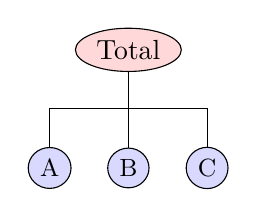
\begin{tikzpicture}
\tikzstyle{every node}=[ellipse,draw,fill=red!15,inner sep=2pt]
\tikzstyle[level distance=.3cm]
\tikzstyle[sibling distance=12cm]
\tikzstyle{level 1}=[sibling distance=10mm,font=\small,set style={{every node}+=[fill=blue!15]}]
\node{Total}[edge from parent fork down]
 child {node {A}
 }
 child {node {B}
 }
 child {node {C}
 };
\end{tikzpicture}
\end{block}
\end{minipage}
\end{textblock}

\begin{textblock}{5.7}(9.4,2.7)\fontsize{14}{15}\sf
\begin{align*}
\bY_{t}&= \begin{pmatrix}
  y_{\text{Total},t}\\
  y_{A,t}\\
  y_{B,t}\\
  y_{C,t}
  \end{pmatrix}  \\
  &= {\color{blue}\underbrace{\begin{pmatrix}
                1 & 1 & 1 \\
                1 & 0 & 0 \\
                0 & 1 & 0\\
                0 & 0 & 1
                \end{pmatrix}}_{\bS}}
     {\color{red}\underbrace{\begin{pmatrix}
       y_{A,t}\\y_{B,t}\\y_{C,t}
       \end{pmatrix}}_{\bm{b}_{t}}}
\end{align*}
\end{textblock}
\end{frame}

\begin{frame}{Temporal constraints: monthly data}
\phantomsection\label{temporal-constraints-monthly-data}
\only<1>{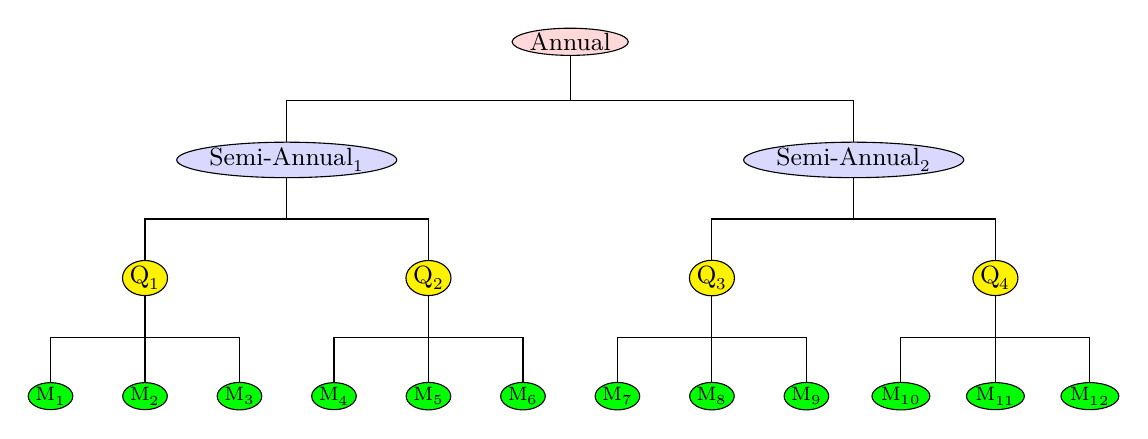
\begin{tikzpicture}
  \tikzstyle{every node}=[ellipse,draw,inner sep=0.2pt,fill=red!15,font=\small]
  \tikzstyle[level distance=.1cm]
  \tikzstyle[sibling distance=7cm]
  \tikzstyle{level 1}=[sibling distance=72mm,set style={{every node}+=[fill=blue!15]}]
  \tikzstyle{level 2}=[sibling distance=36mm,set style={{every node}+=[fill=yellow]}]
  \tikzstyle{level 3}=[sibling distance=12mm,font=\scriptsize,set style={{every node}+=[fill=green]}]
  \node{Annual}[edge from parent fork down]
  child {node {Semi-Annual$_1$}
      child {node {Q$_1$}
          child {node {\scriptsize M$_1$}}
          child {node {\scriptsize M$_2$}}
          child {node {\scriptsize M$_3$}}
        }
      child {node {Q$_2$}
          child {node {\scriptsize M$_4$}}
          child {node {\scriptsize M$_5$}}
          child {node {\scriptsize M$_6$}}
        }
    }
  child {node {Semi-Annual$_2$}
      child {node {Q$_3$}
          child {node {\scriptsize M$_7$}}
          child {node {\scriptsize M$_8$}}
          child {node {\scriptsize M$_9$}}
        }
      child {node {Q$_4$}
          child {node {\scriptsize M$_{10}$}}
          child {node {\scriptsize M$_{11}$}}
          child {node {\scriptsize M$_{12}$}}
        }
    };
\end{tikzpicture}}
\only<2->{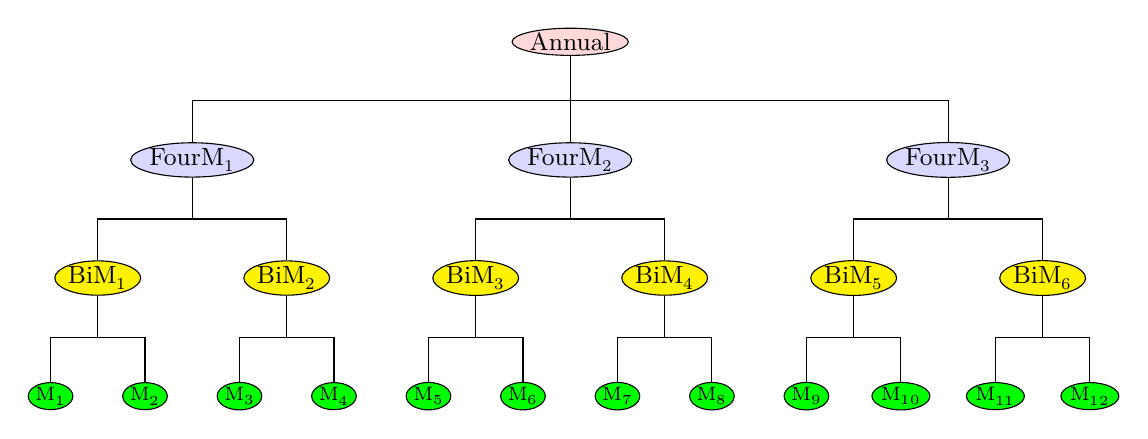
\begin{tikzpicture}
  \tikzstyle{every node}=[ellipse,draw,inner sep=0.2pt,fill=red!15,font=\small]
  \tikzstyle[level distance=.1cm]
  \tikzstyle[sibling distance=7cm]
  \tikzstyle{level 1}=[sibling distance=48mm,set style={{every node}+=[fill=blue!15]}]
  \tikzstyle{level 2}=[sibling distance=24mm,set style={{every node}+=[fill=yellow]}]
  \tikzstyle{level 3}=[sibling distance=12mm,set style={{every node}+=[fill=green]}]
  \node{Annual}[edge from parent fork down]
  child {node {FourM$_1$}
      child {node {BiM$_1$}
          child {node {\scriptsize M$_1$}}
          child {node {\scriptsize M$_2$}}
        }
      child {node {BiM$_2$}
          child {node {\scriptsize M$_3$}}
          child {node {\scriptsize M$_4$}}
        }
    }
  child {node {FourM$_2$}
      child {node {BiM$_3$}
          child {node {\scriptsize M$_5$}}
          child {node {\scriptsize M$_6$}}
        }
      child {node {BiM$_4$}
          child {node {\scriptsize M$_7$}}
          child {node {\scriptsize M$_8$}}
        }
    }
  child {node {FourM$_3$}
      child {node {BiM$_5$}
          child {node {\scriptsize M$_9$}}
          child {node {\scriptsize M$_{10}$}}
        }
      child {node {BiM$_6$}
          child {node {\scriptsize M$_{11}$}}
          child {node {\scriptsize M$_{12}$}}
        }
    };
\end{tikzpicture}}\pause
\end{frame}

\begin{frame}{Temporal constraints: monthly data}
\phantomsection\label{temporal-constraints-monthly-data-1}
\fontsize{11}{11}\sf

\[
  \bm{y}_\tau=\begin{bmatrix}
    x_{\tau}^{[12]}     \\[0.2cm]
    \bm{x}_{\tau}^{[6]} \\[0.2cm]
    \bm{x}_{\tau}^{[4]} \\[0.2cm]
    \bm{x}_{\tau}^{[3]} \\[0.2cm]
    \bm{x}_\tau^{[2]}   \\[0.2cm]
    \bm{x}_\tau^{[1]}
  \end{bmatrix}
  \qquad
  \bm{S}_{te} = \begin{bmatrix}
    1                & 1 & 1 & 1 & 1~~~1~~~1~~~1 & 1 & 1 & 1 & 1 \\
    1                & 1 & 1 & 1 & 1~~~1~~~0~~~0 & 0 & 0 & 0 & 0 \\
    0                & 0 & 0 & 0 & 0~~~0~~~1~~~1 & 1 & 1 & 1 & 1 \\
    1                & 1 & 1 & 1 & 0~~~0~~~0~~~0 & 0 & 0 & 0 & 0 \\
    0                & 0 & 0 & 0 & 1~~~1~~~1~~~1 & 0 & 0 & 0 & 0 \\
    0                & 0 & 0 & 0 & 0~~~0~~~0~~~0 & 1 & 1 & 1 & 1 \\
    1                & 1 & 1 & 0 & 0~~~0~~~0~~~0 & 0 & 0 & 0 & 0 \\
                     &   &   &   & \vdots        &   &   &   &   \\
    0                & 0 & 0 & 0 & 0~~~0~~~0~~~0 & 0 & 1 & 1 & 1 \\
    1                & 1 & 0 & 0 & 0~~~0~~~0~~~0 & 0 & 0 & 0 & 0 \\
                     &   &   &   & \vdots        &   &   &   &   \\
    0                & 0 & 0 & 0 & 0~~~0~~~0~~~0 & 0 & 0 & 1 & 1 \\[0.2cm]
    \phantom{\vdots} &   &   &   & \bm{I}_{12}   &   &   &   &
  \end{bmatrix}
  \qquad
  \bm{b}_\tau = \bm{x}_{\tau}^{[1]} =
  \begin{bmatrix}
   y_{12\tau -11} \\
    y_{12\tau -10} \\
    \vdots        \\
    y_{12\tau}
    \end{bmatrix}
\]
\end{frame}

\section{Optimal linear forecast
reconciliation}\label{optimal-linear-forecast-reconciliation}

\begin{frame}{The coherent subspace}
\phantomsection\label{the-coherent-subspace}
\begin{textblock}{9}(.2,1)\fontsize{13}{13}\sf
\begin{block}{Coherent subspace}
$n_b$-dimensional linear subspace $\mathfrak{s}\subset \mathbb{\chi}^n$ for which linear constraints hold for all $\bm{y}\in\mathfrak{s}$.
\end{block}\vspace*{-0.3cm}
\begin{block}{Hierarchical time series}
An $n$-dimensional multivariate time series such that $\bm{y}_t\in\mathfrak{s}\quad\forall t$.
\end{block}\vspace*{-0.3cm}
\begin{block}{Coherent point forecasts}
$\tilde{\bm{y}}_{t+h|t}$ is \emph{coherent} if $\tilde{\bm{y}}_{t+h|t} \in \mathfrak{s}$.
\end{block}\vspace*{-0.2cm}
\end{textblock}
\only<2-3>{\begin{textblock}{7.5}(.2,6.75)\fontsize{13}{13}\sf
\begin{alertblock}{Base forecasts}
Let $\hat{\bm{y}}_{t+h|t}$ be vector of \emph{incoherent} initial $h$-step forecasts.$\phantom{y_{t|h}}$
\end{alertblock}
\end{textblock}}
\only<3>{\begin{textblock}{7.5}(8.3,6.75)\fontsize{13}{13}\sf
\begin{alertblock}{Reconciled forecasts}
Let $\bm{M}$ be a projection matrix. $\tilde{\bm{y}}_{t+h|t}=\bm{M}\hat{\bm{y}}_{t+h|t}$ ``reconciles'' $\hat{\bm{y}}_{t+h|t}$.
\end{alertblock}
\end{textblock}}

\placefig{9.4}{.0}{width=6.6cm}{3D_hierarchy}
\begin{textblock}{3}(11.4,5.6)\fontsize{13}{13}\sf
\begin{block}{}
\centerline{$y_{Tot} = y_A + y_B$}
\end{block}
\end{textblock}
\end{frame}

\begin{frame}{Minimum trace reconciliation}
\phantomsection\label{minimum-trace-reconciliation}
\begin{textblock}{6.4}(9,-0.1)\begin{block}{}
Wickramasuriya et al (2019)
\end{block}\end{textblock}

\fontsize{14}{15}\sf

\begin{block}{}
\centerline{$\displaystyle\textcolor{red}{\tilde{\by}_{T+h|T}}
= \bm{M} ~ \textcolor{blue}{\hat{\by}_{T+h|T}}$}
\end{block}\vspace*{-0.2cm}
\centerline{\hspace*{1.4cm}\textcolor{red}{Reconciled forecasts}\hfill\textcolor{blue}{Base forecasts}\hspace*{2.9cm}}\vspace*{-0.2cm}

\begin{itemize}
\tightlist
\item
  \(\bm{W}_h = \var[\by_{T+h} - \hat{\by}_{T+h|T} \mid \by_1,\dots,\by_T]\).
\item
  \(\bm{V}_h = \var[\by_{T+h} - \tilde{\by}_{T+h|T} \mid \by_1,\dots,\by_T]) = \bm{M}\bm{W}_h\bm{M}'\).
\end{itemize}

\begin{alertblock}{Minimum trace (MinT) reconciliation}
If $\bm{M}$ is a projection, then trace of $\bm{V}_h$ is minimized when
\centerline{$\bm{M} = \bS(\bS'\bm{W}_h^{-1}\bS)^{-1}\bS'\bm{W}_h^{-1}$}
\end{alertblock}\vspace*{-0.2cm}

\begin{itemize}
\tightlist
\item
  Trace of \(\bm{V}_h\) is sum of forecast variances.
\item
  MinT is \(L_2\) optimal amongst linear unbiased forecasts.
\item
  Several estimates of
  \(\bm{W}_h = \var[\by_{T+h} - \hat{\by}_{T+h|T} \mid \by_1,\dots,\by_T]\)
  have been proposed.
\end{itemize}
\end{frame}

\section{Probabilistic forecast
reconciliation}\label{probabilistic-forecast-reconciliation}

\begin{frame}{The coherent subspace}
\phantomsection\label{the-coherent-subspace-1}
\begin{textblock}{9}(.2,1)\fontsize{13}{13}\sf
\begin{block}{Coherent subspace}
$m$-dimensional linear subspace $\mathfrak{s}\subset \mathbb{\chi}^n$ for which linear constraints hold for all $\bm{y}\in\mathfrak{s}$.
\end{block}\vspace*{-0.3cm}
\begin{block}{Hierarchical time series}
An $n$-dimensional multivariate time series such that $\bm{y}_t\in\mathfrak{s}\quad\forall t$.
\end{block}\vspace*{-0.3cm}
\begin{block}{Coherent point forecasts}
$\tilde{\bm{y}}_{t+h|t}$ is \emph{coherent} if $\tilde{\bm{y}}_{t+h|t} \in \mathfrak{s}$.
\end{block}\vspace*{-0.2cm}
\end{textblock}

\{

\begin{textblock}{7.5}(.2,6.75)\fontsize{13}{13}\sf
\begin{alertblock}{Base forecasts}
Let $\hat{\bm{y}}_{t+h|t}$ be vector of \emph{incoherent} initial $h$-step forecasts.$\phantom{y_{t|h}}$
\end{alertblock}
\end{textblock}

\} \{

\begin{textblock}{7.5}(8.3,6.75)\fontsize{13}{13}\sf
\begin{alertblock}{Reconciled forecasts}
$\tilde{\bm{y}}_{t+h|t}=\bm{M}\hat{\bm{y}}_{t+h|t}$ ``reconciles'' $\hat{\bm{y}}_{t+h|t}$.
\end{alertblock}
\end{textblock}

\}

\placefig{9.4}{.0}{width=6.6cm}{3D_hierarchy}
\begin{textblock}{3}(11.4,5.6)\fontsize{13}{13}\sf
\begin{block}{}
\centerline{$ y_{Tot} = y_A + y_B$}
\end{block}
\end{textblock}
\end{frame}

\begin{frame}{Coherent probabilistic forecasts}
\phantomsection\label{coherent-probabilistic-forecasts}
\begin{textblock}{9.5}(0.2,1)\fontsize{13}{14}\sf
\begin{block}{Coherent probabilistic forecasts}
A probability triple $(\mathfrak{s}, \mathscr{F}_{\mathfrak{s}}, \breve{\nu})$ is coherent with the bottom probability triple $(\mathbb{\chi}^m, \mathscr{F}_{\mathbb{\chi}^m}, \nu)$, if
\centerline{$\breve{\nu}(s(\mathcal{B})) = \nu(\mathcal{B}) \quad \forall \mathcal{B} \in \mathscr{F}_{\mathbb{\chi}^m}$}
\end{block}\vspace*{-0.2cm}
\begin{itemize}\tightlist
\item Random draws from coherent distribution must lie on $\mathfrak{s}$.
\item The probability of points not on $\mathfrak{s}$ is zero.
\item The reconciled distribution is a transformation of the base forecast distribution that is coherent on $\mathfrak{s}$.
\end{itemize}
\end{textblock}
\begin{textblock}{7}(9.5,1.2)
\resizebox{\textwidth}{!}{
\input figs/probforerec_schematic.tex
}
\end{textblock}
\begin{textblock}{7}(9.5,7.5)
\centerline{$\psi = s \circ g$}
\end{textblock}
\begin{textblock}{13.2}(0.2,7.9)
\begin{block}{}\fontsize{12}{12}\sf
\citet{coherentprob,CorEtAl2022}
\end{block}
\end{textblock}
\end{frame}

\begin{frame}{Simulation from a reconciled distribution}
\phantomsection\label{simulation-from-a-reconciled-distribution}
\begin{block}{}
Suppose that $\left(\hat{\bm{y}}^{[1]},\ldots,\hat{\bm{y}}^{[L]}\right)$ is a sample drawn from an incoherent probability measure $\hat{\nu}$. Then $\left(\tilde{\bm{y}}^{[1]},\ldots,\tilde{\bm{y}}^{[L]}\right)$ where $\tilde{\bm{y}}^{[\ell]}:=\psi(\hat{\bm{y}}^{[\ell]})$ for $\ell=1,\ldots,L$, is a sample drawn from the reconciled probability measure $\tilde{\nu}$.
\end{block}\vspace*{-0.4cm}

\begin{itemize}
\tightlist
\item
  Simulate future sample paths for each series, by simulating from each
  model using a multivariate bootstrap of the residuals (to preserve
  cross-correlations).
\item
  Reconcile the sample paths.
\item
  The reconciled sample paths are a sample from the reconciled
  distribution.
\end{itemize}
\end{frame}

\section{Cross-temporal probabilistic forecast
reconciliation}\label{cross-temporal-probabilistic-forecast-reconciliation}

\begin{frame}{Cross-temporal probabilistic forecast reconciliation}
\phantomsection\label{cross-temporal-probabilistic-forecast-reconciliation-1}
\alert{Nonparametric bootstrap}\fontsize{14}{16}\sf

\begin{itemize}
\tightlist
\item
  Simulate future sample paths from all models using bootstrapped
  residuals, then reconcile them to obtain coherent sample paths.
\item
  Need to generate samples that preserve cross-temporal relationships.
\item
  Draw residual samples of all series at same time from most temporally
  aggregated level.
\item
  Residuals for other levels obtained using the corresponding time
  indices.
\end{itemize}
\end{frame}

\begin{frame}{Cross-temporal probabilistic forecast reconciliation}
\phantomsection\label{cross-temporal-probabilistic-forecast-reconciliation-2}
\vspace*{-0.2cm}

\hspace*{-0.8cm}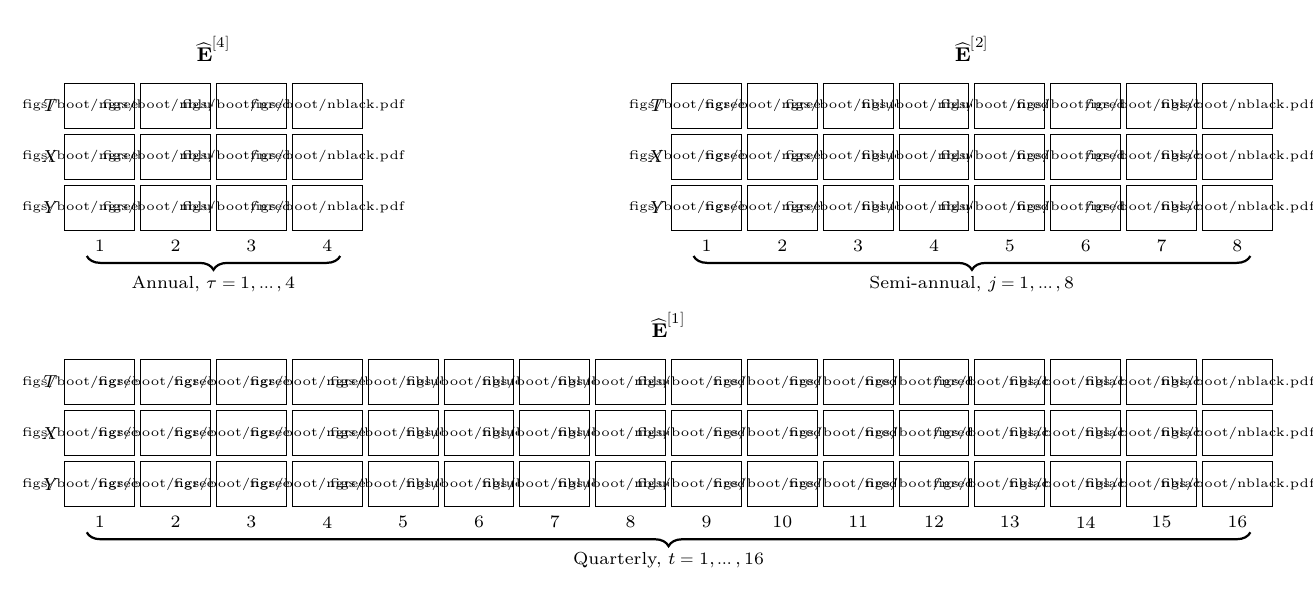
\begin{tikzpicture}[scale = 0.9, every node/.style={scale=0.9}]
\matrix (e1) [matrix of nodes,ampersand replacement=\&,row sep=0cm,column sep=0cm, nodes= {rectangle, fill=white, inner sep = 1pt, font = {\fontsize{7}{6}\selectfont}, minimum width=1em, minimum height=1em,anchor=center}, label={[xshift = 0.5em]above:{\footnotesize$\widehat{\textbf{E}}^{[1]}$}}]
{
$T$ \& \pgfuseimage{ngreen} \& \pgfuseimage{ngreen} \& \pgfuseimage{ngreen} \& \pgfuseimage{ngreen} \& \pgfuseimage{nblue} \& \pgfuseimage{nblue} \& \pgfuseimage{nblue} \& \pgfuseimage{nblue} \& \pgfuseimage{nred} \& \pgfuseimage{nred} \& \pgfuseimage{nred} \& \pgfuseimage{nred} \& \pgfuseimage{nblack} \& \pgfuseimage{nblack} \& \pgfuseimage{nblack} \& \pgfuseimage{nblack} \& \\
$X$ \& \pgfuseimage{ngreen} \& \pgfuseimage{ngreen} \& \pgfuseimage{ngreen} \& \pgfuseimage{ngreen} \& \pgfuseimage{nblue} \& \pgfuseimage{nblue} \& \pgfuseimage{nblue} \& \pgfuseimage{nblue} \& \pgfuseimage{nred} \& \pgfuseimage{nred} \& \pgfuseimage{nred} \& \pgfuseimage{nred} \& \pgfuseimage{nblack} \& \pgfuseimage{nblack} \& \pgfuseimage{nblack} \& \pgfuseimage{nblack} \& \\
$Y$ \& \pgfuseimage{ngreen} \& \pgfuseimage{ngreen} \& \pgfuseimage{ngreen} \& \pgfuseimage{ngreen} \& \pgfuseimage{nblue} \& \pgfuseimage{nblue} \& \pgfuseimage{nblue} \& \pgfuseimage{nblue} \& \pgfuseimage{nred} \& \pgfuseimage{nred} \& \pgfuseimage{nred} \& \pgfuseimage{nred} \& \pgfuseimage{nblack} \& \pgfuseimage{nblack} \& \pgfuseimage{nblack} \& \pgfuseimage{nblack} \& \\
\&  1\&  2\&  3\&  4\&  5\&  6\&  7\&  8\&  9\&  10\&  11\&  12\&  13\&  14\&  15\&  16\\
};
\draw[decorate,thick, decoration={brace, mirror, amplitude=5pt,raise=-1pt}] (e1-4-2.south west) -- (e1-4-17.south east) node[midway, font = {\fontsize{7}{6}\selectfont}, yshift = -1em]{Quarterly, $t = 1,\dots,16$};
\matrix (ek) [above= 10mm of e1.north east, anchor=south east, matrix of nodes,ampersand replacement=\&,row sep=0cm,column sep=0cm, nodes= {rectangle, fill=white, inner sep = 1pt, font = {\fontsize{7}{6}\selectfont}, minimum width=1em, minimum height=1em,anchor=center}, label={[xshift = 0.5em]above:{\footnotesize$\widehat{\textbf{E}}^{[2]}$}}]
{
$T$ \& \pgfuseimage{ngreen} \& \pgfuseimage{ngreen} \& \pgfuseimage{nblue} \& \pgfuseimage{nblue} \& \pgfuseimage{nred} \& \pgfuseimage{nred} \& \pgfuseimage{nblack} \& \pgfuseimage{nblack} \& \\
$X$ \& \pgfuseimage{ngreen} \& \pgfuseimage{ngreen} \& \pgfuseimage{nblue} \& \pgfuseimage{nblue} \& \pgfuseimage{nred} \& \pgfuseimage{nred} \& \pgfuseimage{nblack} \& \pgfuseimage{nblack} \& \\
$Y$ \& \pgfuseimage{ngreen} \& \pgfuseimage{ngreen} \& \pgfuseimage{nblue} \& \pgfuseimage{nblue} \& \pgfuseimage{nred} \& \pgfuseimage{nred} \& \pgfuseimage{nblack} \& \pgfuseimage{nblack} \& \\
\&  1\&  2\&  3\&  4\&  5\&  6\&  7\&  8\\
};
\draw[decorate,thick, decoration={brace, mirror, amplitude=5pt,raise=-1pt}] (ek-4-2.south west) -- (ek-4-9.south east) node[midway, font = {\fontsize{7}{6}\selectfont}, yshift = -1em]{Semi-annual, $j = 1,\dots,8$};
\matrix (em) [above= 10mm of e1.north west, anchor=south west, matrix of nodes,ampersand replacement=\&,row sep=0cm,column sep=0cm, nodes= {rectangle, fill=white, inner sep = 1pt, font = {\fontsize{7}{6}\selectfont}, minimum width=1em, minimum height=1em,anchor=center}, label={[xshift = 0.5em]above:{\footnotesize$\widehat{\textbf{E}}^{[4]}$}}]
{
$T$ \& \pgfuseimage{ngreen}\& \pgfuseimage{nblue}\& \pgfuseimage{nred}\& \pgfuseimage{nblack}\\
$X$ \& \pgfuseimage{ngreen}\& \pgfuseimage{nblue}\& \pgfuseimage{nred}\& \pgfuseimage{nblack}\\
$Y$ \& \pgfuseimage{ngreen}\& \pgfuseimage{nblue}\& \pgfuseimage{nred}\& \pgfuseimage{nblack}\\
\&  1\&  2\&  3\&  4\\
};
\draw[decorate,thick, decoration={brace, mirror, amplitude=5pt,raise=-1pt}] (em-4-2.south west) -- (em-4-5.south east) node[midway, font = {\fontsize{7}{6}\selectfont}, yshift = -1em]{Annual, $\tau = 1,\dots,4$};
\end{tikzpicture}

\begin{textblock}{1.9}(12.9,5.3)
\begin{block}{}\centering
\textcolor[HTML]{7fb97f}{Year 1}\\
\textcolor[HTML]{7fbcff}{Year 2}\\
\textcolor[HTML]{e87f7f}{Year 3}\\
\textcolor[HTML]{7f7f7f}{Year 4}
\end{block}
\end{textblock}

\begin{textblock}{1.9}(12.9,1.6)
\begin{minipage}{1.9cm}
  \begin{block}{}\centering
    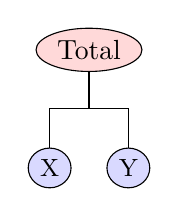
\begin{tikzpicture}
      \tikzstyle{every node}=[ellipse,draw,fill=red!15,inner sep=2pt]
      \tikzstyle[level distance=.3cm]
      \tikzstyle[sibling distance=12cm]
      \tikzstyle{level 1}=[sibling distance=10mm,font=\small,set style={{every node}+=[fill=blue!15]}]
      \node{Total}[edge from parent fork down]
      child {node {X}
        }
      child {node {Y}
        };
    \end{tikzpicture}
  \end{block}
\end{minipage}
\end{textblock}

\begin{textblock}{3}(3.5,1.2)\alert{Data}\end{textblock}
\end{frame}

\begin{frame}{Cross-temporal probabilistic forecast reconciliation}
\phantomsection\label{cross-temporal-probabilistic-forecast-reconciliation-3}
\vspace*{-0.2cm}

\hspace*{-0.8cm}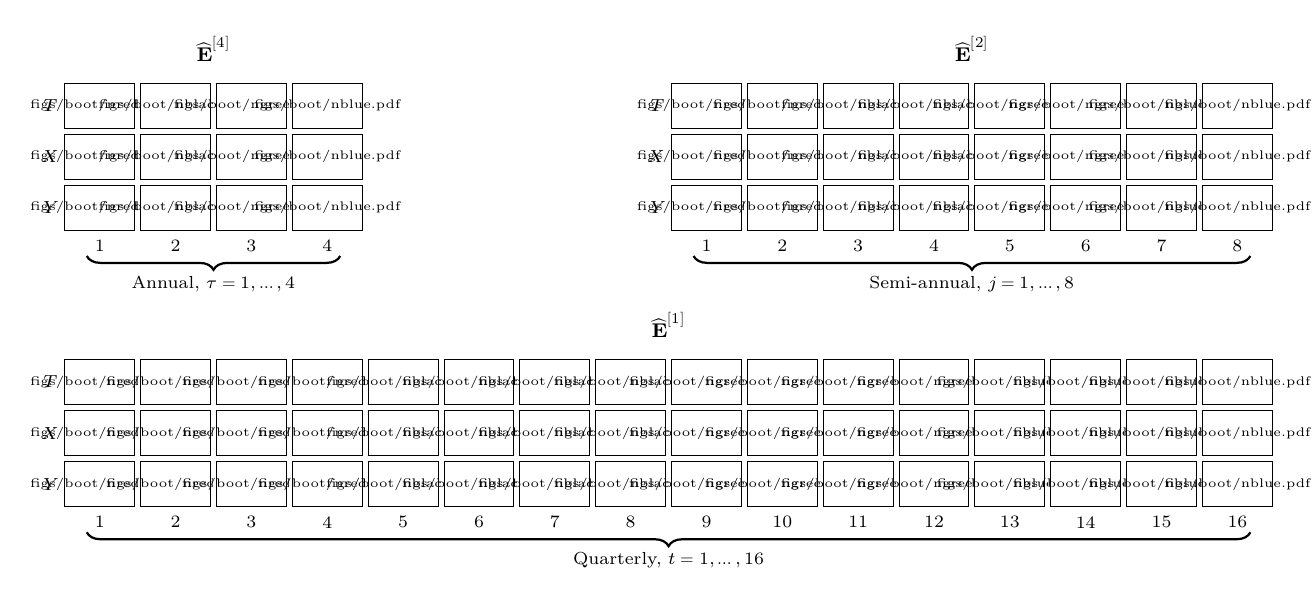
\begin{tikzpicture}[scale = 0.9, every node/.style={scale=0.9}]
\matrix (e1) [matrix of nodes,ampersand replacement=\&,row sep=0cm,column sep=0cm, nodes= {rectangle, fill=white, inner sep = 1pt, font = {\fontsize{7}{6}\selectfont}, minimum width=1em, minimum height=1em,anchor=center}, label={[xshift = 0.5em]above:{\footnotesize$\widehat{\textbf{E}}^{[1]}$}}]
{
$T$ \& \pgfuseimage{nred} \& \pgfuseimage{nred} \& \pgfuseimage{nred} \& \pgfuseimage{nred} \& \pgfuseimage{nblack} \& \pgfuseimage{nblack} \& \pgfuseimage{nblack} \& \pgfuseimage{nblack} \& \pgfuseimage{ngreen} \& \pgfuseimage{ngreen} \& \pgfuseimage{ngreen} \& \pgfuseimage{ngreen} \& \pgfuseimage{nblue} \& \pgfuseimage{nblue} \& \pgfuseimage{nblue} \& \pgfuseimage{nblue} \& \\
$X$ \& \pgfuseimage{nred} \& \pgfuseimage{nred} \& \pgfuseimage{nred} \& \pgfuseimage{nred} \& \pgfuseimage{nblack} \& \pgfuseimage{nblack} \& \pgfuseimage{nblack} \& \pgfuseimage{nblack} \& \pgfuseimage{ngreen} \& \pgfuseimage{ngreen} \& \pgfuseimage{ngreen} \& \pgfuseimage{ngreen} \& \pgfuseimage{nblue} \& \pgfuseimage{nblue} \& \pgfuseimage{nblue} \& \pgfuseimage{nblue} \& \\
$Y$ \& \pgfuseimage{nred} \& \pgfuseimage{nred} \& \pgfuseimage{nred} \& \pgfuseimage{nred} \& \pgfuseimage{nblack} \& \pgfuseimage{nblack} \& \pgfuseimage{nblack} \& \pgfuseimage{nblack} \& \pgfuseimage{ngreen} \& \pgfuseimage{ngreen} \& \pgfuseimage{ngreen} \& \pgfuseimage{ngreen} \& \pgfuseimage{nblue} \& \pgfuseimage{nblue} \& \pgfuseimage{nblue} \& \pgfuseimage{nblue} \& \\
\&  1\&  2\&  3\&  4\&  5\&  6\&  7\&  8\&  9\&  10\&  11\&  12\&  13\&  14\&  15\&  16\\
};
\draw[decorate,thick, decoration={brace, mirror, amplitude=5pt,raise=-1pt}] (e1-4-2.south west) -- (e1-4-17.south east) node[midway, font = {\fontsize{7}{6}\selectfont}, yshift = -1em]{Quarterly, $t = 1,\dots,16$};
\matrix (ek) [above= 10mm of e1.north east, anchor=south east, matrix of nodes,ampersand replacement=\&,row sep=0cm,column sep=0cm, nodes= {rectangle, fill=white, inner sep = 1pt, font = {\fontsize{7}{6}\selectfont}, minimum width=1em, minimum height=1em,anchor=center}, label={[xshift = 0.5em]above:{\footnotesize$\widehat{\textbf{E}}^{[2]}$}}]
{
$T$ \& \pgfuseimage{nred} \& \pgfuseimage{nred} \& \pgfuseimage{nblack} \& \pgfuseimage{nblack} \& \pgfuseimage{ngreen} \& \pgfuseimage{ngreen} \& \pgfuseimage{nblue} \& \pgfuseimage{nblue} \& \\
$X$ \& \pgfuseimage{nred} \& \pgfuseimage{nred} \& \pgfuseimage{nblack} \& \pgfuseimage{nblack} \& \pgfuseimage{ngreen} \& \pgfuseimage{ngreen} \& \pgfuseimage{nblue} \& \pgfuseimage{nblue} \& \\
$Y$ \& \pgfuseimage{nred} \& \pgfuseimage{nred} \& \pgfuseimage{nblack} \& \pgfuseimage{nblack} \& \pgfuseimage{ngreen} \& \pgfuseimage{ngreen} \& \pgfuseimage{nblue} \& \pgfuseimage{nblue} \& \\
\&  1\&  2\&  3\&  4\&  5\&  6\&  7\&  8\\
};
\draw[decorate,thick, decoration={brace, mirror, amplitude=5pt,raise=-1pt}] (ek-4-2.south west) -- (ek-4-9.south east) node[midway, font = {\fontsize{7}{6}\selectfont}, yshift = -1em]{Semi-annual, $j = 1,\dots,8$};
\matrix (em) [above= 10mm of e1.north west, anchor=south west, matrix of nodes,ampersand replacement=\&,row sep=0cm,column sep=0cm, nodes= {rectangle, fill=white, inner sep = 1pt, font = {\fontsize{7}{6}\selectfont}, minimum width=1em, minimum height=1em,anchor=center}, label={[xshift = 0.5em]above:{\footnotesize$\widehat{\textbf{E}}^{[4]}$}}]
{
$T$ \& \pgfuseimage{nred}\& \pgfuseimage{nblack}\& \pgfuseimage{ngreen}\& \pgfuseimage{nblue}\\
$X$ \& \pgfuseimage{nred}\& \pgfuseimage{nblack}\& \pgfuseimage{ngreen}\& \pgfuseimage{nblue}\\
$Y$ \& \pgfuseimage{nred}\& \pgfuseimage{nblack}\& \pgfuseimage{ngreen}\& \pgfuseimage{nblue}\\
\&  1\&  2\&  3\&  4\\
};
\draw[decorate,thick, decoration={brace, mirror, amplitude=5pt,raise=-1pt}] (em-4-2.south west) -- (em-4-5.south east) node[midway, font = {\fontsize{7}{6}\selectfont}, yshift = -1em]{Annual, $\tau = 1,\dots,4$};
\end{tikzpicture}

\begin{textblock}{1.9}(12.9,5.3)
\begin{block}{}\centering
\textcolor[HTML]{7fb97f}{Year 1}\\
\textcolor[HTML]{7fbcff}{Year 2}\\
\textcolor[HTML]{e87f7f}{Year 3}\\
\textcolor[HTML]{7f7f7f}{Year 4}
\end{block}
\end{textblock}

\begin{textblock}{1.9}(12.9,1.6)
\begin{minipage}{1.9cm}
  \begin{block}{}\centering
    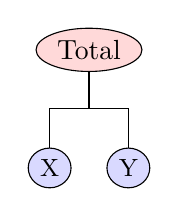
\begin{tikzpicture}
      \tikzstyle{every node}=[ellipse,draw,fill=red!15,inner sep=2pt]
      \tikzstyle[level distance=.3cm]
      \tikzstyle[sibling distance=12cm]
      \tikzstyle{level 1}=[sibling distance=10mm,font=\small,set style={{every node}+=[fill=blue!15]}]
      \node{Total}[edge from parent fork down]
      child {node {X}
        }
      child {node {Y}
        };
    \end{tikzpicture}
  \end{block}
\end{minipage}
\end{textblock}

\begin{textblock}{3}(3.5,1.2)\alert{Bootstrap}\end{textblock}
\end{frame}

\begin{frame}{Cross-temporal probabilistic forecast reconciliation}
\phantomsection\label{cross-temporal-probabilistic-forecast-reconciliation-4}
\vspace*{-0.2cm}

\hspace*{-0.8cm}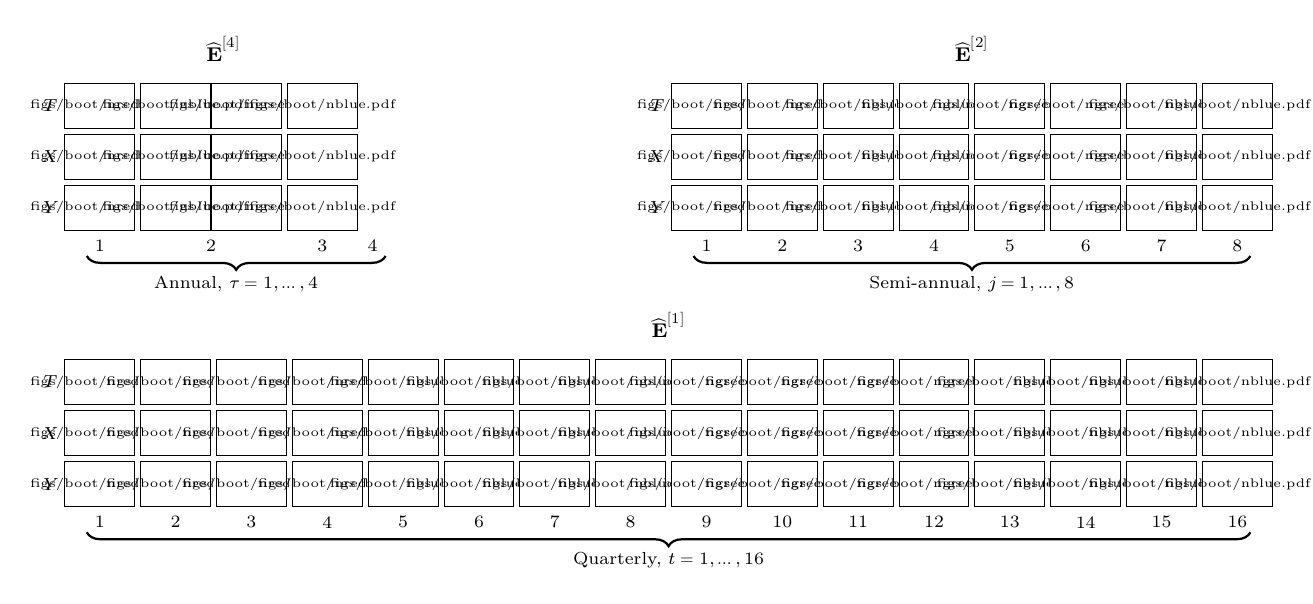
\begin{tikzpicture}[scale = 0.9, every node/.style={scale=0.9}]
\matrix (e1) [matrix of nodes,ampersand replacement=\&,row sep=0cm,column sep=0cm, nodes= {rectangle, fill=white, inner sep = 1pt, font = {\fontsize{7}{6}\selectfont}, minimum width=1em, minimum height=1em,anchor=center}, label={[xshift = 0.5em]above:{\footnotesize$\widehat{\textbf{E}}^{[1]}$}}]
{
$T$ \& \pgfuseimage{nred} \& \pgfuseimage{nred} \& \pgfuseimage{nred} \& \pgfuseimage{nred} \& \pgfuseimage{nblue} \& \pgfuseimage{nblue} \& \pgfuseimage{nblue} \& \pgfuseimage{nblue} \& \pgfuseimage{ngreen} \& \pgfuseimage{ngreen} \& \pgfuseimage{ngreen} \& \pgfuseimage{ngreen} \& \pgfuseimage{nblue} \& \pgfuseimage{nblue} \& \pgfuseimage{nblue} \& \pgfuseimage{nblue} \& \\
$X$ \& \pgfuseimage{nred} \& \pgfuseimage{nred} \& \pgfuseimage{nred} \& \pgfuseimage{nred} \& \pgfuseimage{nblue} \& \pgfuseimage{nblue} \& \pgfuseimage{nblue} \& \pgfuseimage{nblue} \& \pgfuseimage{ngreen} \& \pgfuseimage{ngreen} \& \pgfuseimage{ngreen} \& \pgfuseimage{ngreen} \& \pgfuseimage{nblue} \& \pgfuseimage{nblue} \& \pgfuseimage{nblue} \& \pgfuseimage{nblue} \& \\
$Y$ \& \pgfuseimage{nred} \& \pgfuseimage{nred} \& \pgfuseimage{nred} \& \pgfuseimage{nred} \& \pgfuseimage{nblue} \& \pgfuseimage{nblue} \& \pgfuseimage{nblue} \& \pgfuseimage{nblue} \& \pgfuseimage{ngreen} \& \pgfuseimage{ngreen} \& \pgfuseimage{ngreen} \& \pgfuseimage{ngreen} \& \pgfuseimage{nblue} \& \pgfuseimage{nblue} \& \pgfuseimage{nblue} \& \pgfuseimage{nblue} \& \\
\&  1\&  2\&  3\&  4\&  5\&  6\&  7\&  8\&  9\&  10\&  11\&  12\&  13\&  14\&  15\&  16\\
};
\draw[decorate,thick, decoration={brace, mirror, amplitude=5pt,raise=-1pt}] (e1-4-2.south west) -- (e1-4-17.south east) node[midway, font = {\fontsize{7}{6}\selectfont}, yshift = -1em]{Quarterly, $t = 1,\dots,16$};
\matrix (ek) [above= 10mm of e1.north east, anchor=south east, matrix of nodes,ampersand replacement=\&,row sep=0cm,column sep=0cm, nodes= {rectangle, fill=white, inner sep = 1pt, font = {\fontsize{7}{6}\selectfont}, minimum width=1em, minimum height=1em,anchor=center}, label={[xshift = 0.5em]above:{\footnotesize$\widehat{\textbf{E}}^{[2]}$}}]
{
$T$ \& \pgfuseimage{nred} \& \pgfuseimage{nred} \& \pgfuseimage{nblue} \& \pgfuseimage{nblue} \& \pgfuseimage{ngreen} \& \pgfuseimage{ngreen} \& \pgfuseimage{nblue} \& \pgfuseimage{nblue} \& \\
$X$ \& \pgfuseimage{nred} \& \pgfuseimage{nred} \& \pgfuseimage{nblue} \& \pgfuseimage{nblue} \& \pgfuseimage{ngreen} \& \pgfuseimage{ngreen} \& \pgfuseimage{nblue} \& \pgfuseimage{nblue} \& \\
$Y$ \& \pgfuseimage{nred} \& \pgfuseimage{nred} \& \pgfuseimage{nblue} \& \pgfuseimage{nblue} \& \pgfuseimage{ngreen} \& \pgfuseimage{ngreen} \& \pgfuseimage{nblue} \& \pgfuseimage{nblue} \& \\
\&  1\&  2\&  3\&  4\&  5\&  6\&  7\&  8\\
};
\draw[decorate,thick, decoration={brace, mirror, amplitude=5pt,raise=-1pt}] (ek-4-2.south west) -- (ek-4-9.south east) node[midway, font = {\fontsize{7}{6}\selectfont}, yshift = -1em]{Semi-annual, $j = 1,\dots,8$};
\matrix (em) [above= 10mm of e1.north west, anchor=south west, matrix of nodes,ampersand replacement=\&,row sep=0cm,column sep=0cm, nodes= {rectangle, fill=white, inner sep = 1pt, font = {\fontsize{7}{6}\selectfont}, minimum width=1em, minimum height=1em,anchor=center}, label={[xshift = 0.5em]above:{\footnotesize$\widehat{\textbf{E}}^{[4]}$}}]
{
$T$ \& \pgfuseimage{nred}\& \pgfuseimage{nblue}\pgfuseimage{ngreen}\& \pgfuseimage{nblue}\\
$X$ \& \pgfuseimage{nred}\& \pgfuseimage{nblue}\pgfuseimage{ngreen}\& \pgfuseimage{nblue}\\
$Y$ \& \pgfuseimage{nred}\& \pgfuseimage{nblue}\pgfuseimage{ngreen}\& \pgfuseimage{nblue}\\
\&  1\&  2\&  3\&  4\\
};
\draw[decorate,thick, decoration={brace, mirror, amplitude=5pt,raise=-1pt}] (em-4-2.south west) -- (em-4-5.south east) node[midway, font = {\fontsize{7}{6}\selectfont}, yshift = -1em]{Annual, $\tau = 1,\dots,4$};
\end{tikzpicture}

\begin{textblock}{1.9}(12.9,5.3)
\begin{block}{}\centering
\textcolor[HTML]{7fb97f}{Year 1}\\
\textcolor[HTML]{7fbcff}{Year 2}\\
\textcolor[HTML]{e87f7f}{Year 3}\\
\textcolor[HTML]{7f7f7f}{Year 4}
\end{block}
\end{textblock}

\begin{textblock}{1.9}(12.9,1.6)
\begin{minipage}{1.9cm}
  \begin{block}{}\centering
    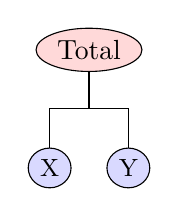
\begin{tikzpicture}
      \tikzstyle{every node}=[ellipse,draw,fill=red!15,inner sep=2pt]
      \tikzstyle[level distance=.3cm]
      \tikzstyle[sibling distance=12cm]
      \tikzstyle{level 1}=[sibling distance=10mm,font=\small,set style={{every node}+=[fill=blue!15]}]
      \node{Total}[edge from parent fork down]
      child {node {X}
        }
      child {node {Y}
        };
    \end{tikzpicture}
  \end{block}
\end{minipage}
\end{textblock}

\begin{textblock}{3}(3.5,1.2)\alert{Bootstrap}\end{textblock}

\only<2>{\begin{textblock}{8}(3.7,4)
\begin{alertblock}{}
The ``year'' can start in any quarter, giving overlapping blocks.
\end{alertblock}
\end{textblock}}
\end{frame}

\begin{frame}{Monthly Australian Tourism Demand}
\phantomsection\label{monthly-australian-tourism-demand}
\begin{textblock}{6}(0.2,1.2)
\centering\fontsize{12}{13}\sf
\textbf{Geographical division}\\
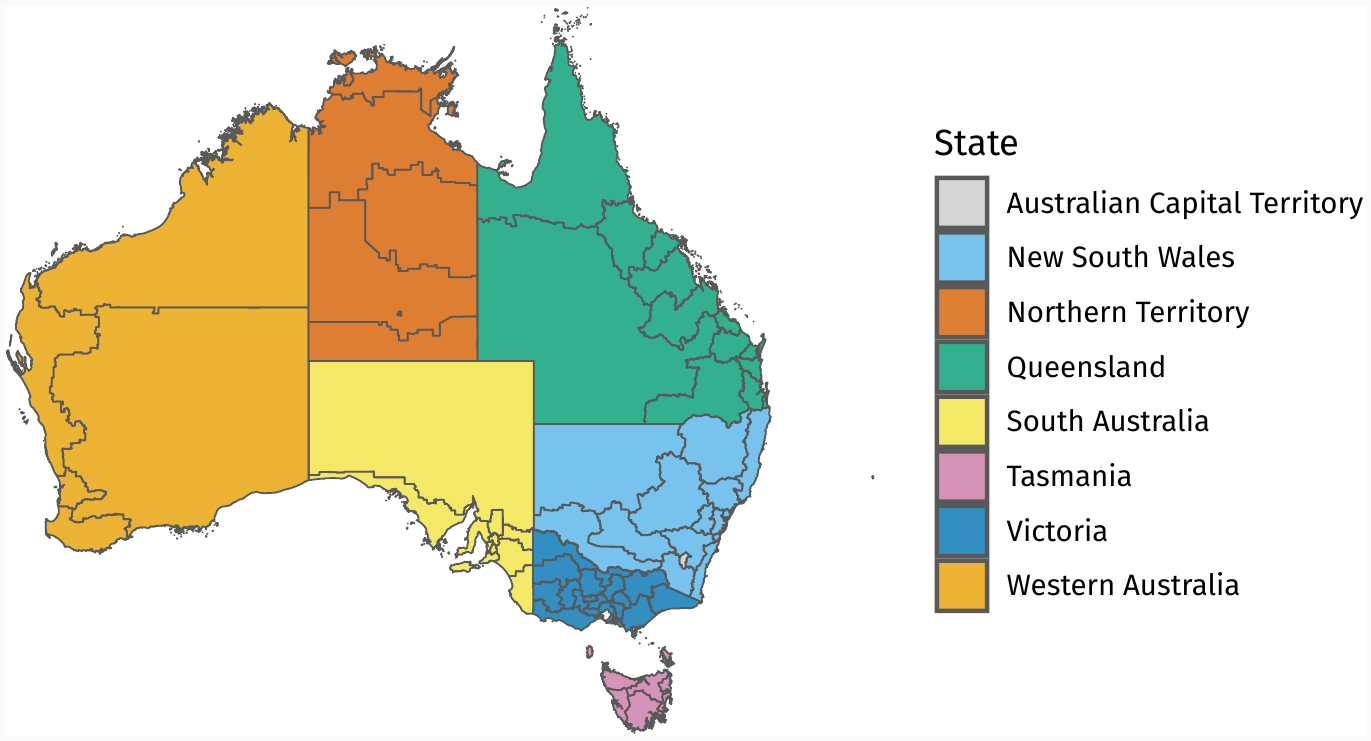
\includegraphics[width = 5.5cm, trim= 0 0 180 0, clip=true]{figs/aus_map}\\[-0.4cm]
\faTimes\\
\textbf{Purpose of travel}\\
{\fontsize{11}{12}\sf Holiday, Visiting friends \& relatives, Business, Other}
\end{textblock}

\begin{textblock}{10}(6.1,1)
\fontsize{11}{14}\sf\tabcolsep=0.12cm
\begin{itemize}
\item \textbf{Grouped ts}\newline (geographical divisions $\times$ purpose of travel)

\begin{tabular}{lccccc}
\toprule
  & \textbf{AUS} & \textbf{States} & \textbf{Zones$^\ast$} & \textbf{Regions} & \textbf{Tot}\\
  \midrule
  \textbf{geographical} & {\color{newblue}1} & {\color{newblue}7} & {\color{newblue}21} & {\color{newblue}76} & 105 \\
  \textbf{purpose} & {\color{newblue}4} & {\color{newblue}28} & {\color{newblue}84} & {\color{avocado}304} & 420\\
  \midrule
  \textbf{total} & 5 & 35 & 105 & 380 & \textbf{525}\\
  \bottomrule
\end{tabular}
\centerline{{\color{newblue}$n_a = 221$}, {\color{avocado}$n_b = 304$}, and $\textbf{n = 525}$}

\item \textbf{Temporal framework}, frequencies:\\[0.2cm]
\begin{multicols}{2}
  \begin{itemize}\tightlist
  \item Monthly
  \item Bi-Monthly
  \item Quarterly
  \end{itemize}
  \begin{itemize}\tightlist
  \item Four-Monthly
  \item Semi-Annual
  \item Annual
  \end{itemize}
\end{multicols}
\end{itemize}
\end{textblock}
\end{frame}

\begin{frame}{Monthly Australian Tourism Demand}
\phantomsection\label{monthly-australian-tourism-demand-1}
\begin{itemize}
\item
  Monthly data: January 1998 to December 2016
\item
  Time series cross-validation; initial training set 10 years.
\item
  One-month increase in each training set
\item
  For each training set, compute temporally aggregated series for
  \(k \in \{1,2,3,4,6,12\}\), and produce forecasts up to \(h_2=6\),
  \(h_3=4\), \(h_4=3\), \(h_6=2\) and \(h_{12}=1\) steps ahead.
\item
  Automatic ETS forecasts on log-transformed data
\end{itemize}
\end{frame}

\begin{frame}{Monthly Australian Tourism Demand}
\phantomsection\label{monthly-australian-tourism-demand-2}
\alert{Reconciliation approaches}\fontsize{13}{14}\sf

\begin{itemize}
\item
  Cross-temporal \textbf{\color{newblue}{bottom-up}} and
  \textbf{\color{newblue}{partly bottom-up}}

  \begin{tabular}{M{0.24\linewidth}|M{0.24\linewidth}|M{0.24\linewidth}}
  ct$(bu)$ & ct$(shr_{cs}, bu_{te})$ & ct$(wlsv_{te}, bu_{cs})$
  \end{tabular}
\item
  Optimal forecast reconciliation with
  \textbf{\color{newblue}{one-step residuals}}

  \begin{tabular}{M{0.24\linewidth}|M{0.24\linewidth}|M{0.24\linewidth}|M{0.24\linewidth}}
    oct$(ols)$ & oct$(struc)$ & oct$(wlsv)$ & oct$(bdshr)$
    \end{tabular}
\item
  Optimal forecast reconciliation with
  \textbf{\color{newblue}{multi-step residuals}}

  \begin{tabular}{M{0.24\linewidth}|M{0.24\linewidth}|M{0.24\linewidth}|M{0.24\linewidth}}
    oct$_h(hbshr)$ & oct$_h(bshr)$ & oct$_h(hshr)$ & oct$_h(shr)$
    \end{tabular}
\end{itemize}
\end{frame}

\begin{frame}{Monthly Australian tourism data -- CRPS skill scores}
\phantomsection\label{monthly-australian-tourism-data-crps-skill-scores}
\fontsize{12}{13}\sf\vspace*{0.2cm}

\centerline{\textcolor{red}{Worse than benchmark}\qquad \textbf{Best}}

\centering
\footnotesize
\begin{tabular}[t]{lrr}
& \textbf{$\forall k \in \{12,6,4,3,2,1\}$} & \textbf{$k = 1$}\\
\midrule
base                      & \cellcolor{LightOrange!30} {1.000}  & \cellcolor{LightOrange!30} {1.000} \\
ct$(bu)$                  & \textcolor{red}{1.321}              & \textcolor{red}{1.077} \\
ct$(shr_{cs}, bu_{te})$   & \textcolor{red}{1.057}              & {0.976} \\
ct$(wlsv_{te}, bu_{cs})$  & \textcolor{red}{1.062}              & {0.976}\\
oct$(ols)$                & {0.989}                             & {0.982}\\
oct$(struc)$              & {0.982}                             & {0.970}\\
oct$(wlsv)$               & {0.987}                             & {0.952} \\
oct$(bdshr)$              & {0.975}                             & {\textbf{0.949}} \\
oct$_h(hbshr)$            & {0.989}                             & {0.982} \\
oct$_h(bshr)$             & {0.994}                             & {0.988}\\
oct$_h(hshr)$             & {\textbf{0.969}}                    & {0.953}\\
oct$_h(shr)$              & \textcolor{red}{1.007}              & \textcolor{red}{1.000}
\end{tabular}
\end{frame}

\section{Final comments}\label{final-comments}

\begin{frame}[fragile]{Software}
\phantomsection\label{software}
\fontsize{11}{12}\sf\vspace*{0.3cm}

\hspace*{-0.6cm}\begin{tabular}{llP{1.7cm}cP{1.7cm}c}
\toprule
Package                                                                      & Language  & Cross-sectional  & Temporal    & Cross-temporal  & Probabilistic\\
\midrule
\texttt{\href{https://pkg.earo.me/hts/}{hts}}
    & R         & \checkmark       &             &                 & \\
\texttt{\href{http://pkg.robjhyndman.com/thief/}{thief}}
    & R         &                  & \checkmark  &                 & \\
\texttt{\href{https://fable.tidyverts.org}{fable}}
    & R         & \checkmark       &             &                 & \checkmark\\
\texttt{\href{https://danigiro.github.io/FoReco/}{FoReco}}
    & R         & \checkmark       & \checkmark  & \checkmark      & \checkmark\\
\texttt{\href{https://angelpone.github.io/pyhts/}{pyhts}}
    & Python    & \checkmark       & \checkmark  &                 & \\
\texttt{\href{https://nixtla.github.io/hierarchicalforecast/}{hierarchicalforecast}}
    & Python    & \checkmark       &             &                 & \checkmark \\
\bottomrule
\end{tabular}

\begin{itemize}
\tightlist
\item
  \texttt{hts}, \texttt{thief}, and \texttt{FoReco} use \texttt{ts}
  objects
\item
  \texttt{fable} uses \texttt{tsibble} objects
\item
  \texttt{fable} has plans to implement temporal and cross-temporal
  reconciliation
\end{itemize}
\end{frame}

\begin{frame}{More information}
\phantomsection\label{more-information}
\fontsize{18}{20}\sf

\href{https://robjhyndman.com}{\faicon{home} robjhyndman.com}

\href{https://aus.social/@robjhyndman}{
\includegraphics[width=0.5cm]{figs/mastodon}\, aus.social/@robjhyndman}

\href{https://github.com/robjhyndman}{\faicon{github}  @robjhyndman}

\href{mailto:rob.hyndman@monash.edu}{\faicon{envelope}  rob.hyndman@monash.edu}

\nocite{hierarchical,fasthts, mint, hfreview, htsgeometry}
\nocite{Di_FonGir2022a,temporal-hierarchies,ctprob}
\end{frame}


\begin{frame}[allowframebreaks]{References}
  \bibliographytrue
  \printbibliography[heading=none]
\end{frame}


\end{document}
